In this section we evaluate the use of search in finding an effective enabling of \verb-par-s that achieves a worthwhile speed-up when the parellelised program is run in a multi-core architecture.  As a reminder, the starting point for our proposed technique is a program that was originally written to be run sequentially on a single core; static analysis identifies potential sites at which \verb-par- functions \emph{could} be applied; and then search is used to determine the subset of sites at which the \verb-par- is actually applied.

% The evaluation is motivated by an intended use-case for the technique: that an effective---not necessary optimal---placement of (\verb-par-s) can be found during the equivalent of a coffee break.

\subsection{Research Questions}

Our hypothesis is that enabling a subset of the \verb-par-s will often be preferable to enabling them all, hence the first research question:\\

\noindent\textbf{RQ1} What speed-up is achieved by using search to enable a subset of \verb-par-s compared to the enabling all the \verb-par-s found by static analysis? \\

Since the overall goal is to speed-up a sequential program by parallelising it to use multiple cores, the second question is:\\

\noindent\textbf{RQ2} What speed-up is achieved by parallelisation using search compared to the original software-under-test (SUT) executed as a sequential program?\\

In this empirical work, we consider two algorithms: a simple hill-climbing algorithm and a greedy algorithm:\\

\noindent\textbf{RQ3} Which search algorithm achieves the larger speed-ups, and how quickly do these algorithms achieve these speed-ups?\\

Since some \verb-par-s can only have an effect when one or more other \verb-par-s are also enabled, there is an argument that a sensible starting point for both algorithms is to have all \verb-par-s enabled.  An alternative is to start with a random subset of the \verb-par-s enabled.  This motivates the final research question:\\

\noindent\textbf{RQ4} Which form of initialisation enables the algorithm to find the best speed-ups: all \verb-par-s enabled (we refer to this as \emph{`all-on'} initialisation), or a random subset enabled (\emph{`random'} initialisation)?

\subsection{Algorithms}

\paragraph{Representation} We represent the choice of enabled \verb-par-s as a bit string where a 1 indicates that the \verb-par- is applied at a site, and 0 that it is not.  The length of the bit string is the number of potential \verb-par-s annotations found by the static analysis.

\paragraph{Fitness} To facilitate experimentation, the SUTs are executed using a simulator which records the number of reductions made by each thread.  A parameter to the simulator controls the number of cores available to the SUT, and thus the maximum number of threads that may be run in parallel.  We choose the number of reductions made by the main thread as the fitness metric. The main thread cannot complete until all the other threads it has started have completed, and so this number of reductions is an indication of the SUT's runtime.  The simulator includes a realistic overhead of 250 reductions for handling each additional thread.
% The number of reductions made by the main thread is not the total number of reductions made by the SUT unless the SUT is sequential: if it has been parallelised, many of the reductions will be performed on other threads.

\paragraph{Hill-Climbing Algorithm} We utilise a simple hill-climbing algorithm in which the neighbours of the current bitstring are those formed by flipping a single bit.  At each iteration, these neighbours of the current bitstring are considered in a random order, and the fitness evaluated for each in turn. The first neighbour that has a better fitness, i.e.~fewer reductions are made by the main thread, than the current bitstring becomes the current bitstring in the next iteration.  The algorithm terminates when no neighbour of the current bitstring has a better fitness.

\paragraph{Greedy Algorithm} The greedy algorithm considers the bits in representation in a random order.  As each bit is considered, the bit is flipped from its current setting and the resulting bit string evaluated; the setting of the bit---current or flipped---with the better fitness is retained.  The algorithm terminates once all the bits have been evaluated.

\subsection{Software-Under-Test}

\paragraph{SumEuler}
SumEuler is a common parallel functional programming benchmark first introduced
with the work on the $\langle\nu, G\rangle$-Machine in 1989 \citep{vGMachine}.
This program is often used a parallel compiler benchmark making it a `sanity-check'
for our work. We expect to see consistent speed-ups in this program when parallelised (9 \verb-par- sites).

\paragraph{Queens $+$ Queens2}
We benchmark two versions of the nQueens program. Queens2 is a purely symbolic
version that represents the board as a list of lists and does not perform
numeric computation (10 \verb-par- sites for Queens and 24 for Queens2). The fact
that Queens2 has more than double the number of \verb-par- sites for the same
problem shows that writing in a more symbolic style provides more opportunity
for \emph{safe} parallelism.

\paragraph{SodaCount}
Solves a word search problem for a given grid of letters
and a list of keywords.  Introduced by Runciman and Wakeling, this program was
chosen because it exhibits a standard search problem and because Runciman and
Wakeling hand-tuned and profiled a parallel version, demonstrating
that impressive speed-ups are possible with this program
\citep{Runciman:1996:AFP:242105} (15 \verb-par- sites).

\paragraph{Tak}
Small recursive numeric computation that calculates a Takeuchi number. Knuth
describes the properties of Tak in \citep{ExamplesOfRecursion} (2 \verb-par- sites).

\paragraph{Taut}
Determines whether a given predicate expression is a tautology. This program
was chosen because the algorithm used is \emph{inherently sequential}. We feel
that it was important to demonstrate that not all programs have implicit parallelism
within them, sometimes the only way to achieve parallel speed-ups is to rework
the algorithm (15 \verb-par- sites).

\paragraph{MatMul}
List of list matrix multiplication. Matrix multiplication is an inherently parallel
operation, we expect this program to demonstrate speed-ups when parallelised (7 \verb-par- sites).

\subsection{Method}

The following four algorithm configurations were evaluated:
\begin{itemize}
	\item hill-climbing with all-on initialisation
	\item greedy with all-on initialisation
	\item hill-climbing with random initialisation
	\item greedy with random initialisation
\end{itemize}

Each algorithm configuration was evaluated for four settings of the number cores: 4, 8, 16 and 24 cores. Each algorithm / core count combination was evaluated against each of the seven SUTs described above.

Since both search algorithms are stochastic, multiple runs were made for each algorithm / core count / SUT combination, each using 30 different seeds to the pseudo-random number generator.  For all runs, after each fitness evaluation, the best bit string found and its fitness (the number of reductions made by the main thread), was recorded.

In addition, the fitness (number of reductions) was evaluated for a bit string where all bits are set to 1: this equivalent to using the static analysis without optimisation using search.  This evaluation was made for each combination of core count and SUT.  Finally, the fitness was evaluated for the sequential version of each SUT.

\subsection{Results}

The results are summarised in table~\ref{tab:speedups}.  This table compares the speed-up, calculated as the ratio of the medians of the reduction counts, of hill-climbing with all-on initialisation compared to (a) the parallelisation that would result from the static analysis without optimisation; (b) the sequential version of the program; (c) the greedy algorithm with all-on initialisation; and (d) the hill-climbing algorithm with random initialisation.  The speed-up is calculated as the factor by which the number of reductions is reduced, and so values greater than 1 indicate that the SUT parallelised using hill-climbing with all-on initialisation would be faster in the multi-core environment.  Values in bold in the table indicate that differences between the algorithms used to calculate the speed-up are statistically significant at the 5\% level using a one- or two-sample Wilcoxon test as appropriate\footnote{Since in the following we discuss the results for each SUT, or combination of SUT and number of cores, individually as well as for the entire set of results as a family, we do not apply a Bonferroni or similar correction to the significance level.  Nevertheless we note here that most of the currently significant differences would remain significant if such a correction were applied.}.

\begin{table}
\centering
	\sisetup{detect-weight=true, detect-inline-weight=math,round-mode=figures, round-precision=4}
\begin{tabular}{c|c|S|S|S|S}
% 	& & \multicolumn{3}{c|}{HC random init vs.} & \multicolumn{3}{c|}{HC all-on init vs.} & random init \\
% SUT & cores & parallel & sequential & greedy & parallel & sequential & greedy & vs. all on \\ \hline
 	& & \multicolumn{4}{c}{hill-climbing speed-up compared to:} \\
 SUT & {cores} & {\parbox{2cm}{\centering static parallel}} & {\parbox{2cm}{\centering sequential}} & {\parbox{2cm}{\centering greedy}} & {\parbox{2cm}{\centering random init}} \\ \hline
MatMul & 4 & \bfseries 4.90301661707919  & \bfseries 1.02124759973798  &  1  &  1  \\
MatMul & 8 & \bfseries 4.62464276508472  & \bfseries 1.02124759973798  &  1  &  1  \\
MatMul & 16 & \bfseries 4.48549626511679  & \bfseries 1.02124759973798  &  1  &  1  \\
MatMul & 24 & \bfseries 4.43914308383459  & \bfseries 1.02124759973798  &  1  &  1  \\
Queens & 4 & \bfseries 1.08002338656061  & \bfseries 1.29449651880535  &  1  &  1  \\
Queens & 8 & \bfseries 1.04284123826334  & \bfseries 1.36903090592333  &  1  &  1  \\
Queens & 16 & \bfseries 1.01658424583816  & \bfseries 1.40075887342919  &  1  &  1  \\
Queens & 24 & \bfseries 1.00284839597168  & \bfseries 1.40077452594306  & \bfseries 1.000005587155  &  1  \\
Queens2 & 4 & \bfseries 6.47871841266272  & \bfseries 3.84268026498045  &  1  &  1  \\
Queens2 & 8 & \bfseries 6.4214444887208  & \bfseries 7.60677419801831  &  1  &  1  \\
Queens2 & 16 & \bfseries 6.26286318030988  & \bfseries 14.7914211715831  &  1  &  1  \\
Queens2 & 24 & \bfseries 6.10111087862129  & \bfseries 21.5370475166917  &  1  &  1  \\
SodaCount & 4 & \bfseries 4.23709552156544  & \bfseries 3.77256127760359  & \bfseries 1.00090381935946  & \bfseries 1.05522740981559  \\
SodaCount & 8 & \bfseries 3.54406724309037  & \bfseries 6.20691010897515  & \bfseries 1.00698493625413  & \bfseries 1.07054373432511  \\
SodaCount & 16 & \bfseries 3.10964257836354  & \bfseries 10.3951019801297  & \bfseries 1.08075042082402  & \bfseries 1.07197550990065  \\
SodaCount & 24 & \bfseries 2.80981399852391  & \bfseries 13.2551680242675  & \bfseries 1.00369023678455  &  1  \\
SumEuler & 4 & \bfseries 1.49372579894484  & \bfseries 3.94797162309201  &  1  &  1  \\
SumEuler & 8 & \bfseries 1.48574818274656  & \bfseries 7.77250594496659  &  1  &  1  \\
SumEuler & 16 & \bfseries 1.46021192398224  & \bfseries 14.7739589421968  & \bfseries 1  &  1  \\
SumEuler & 24 & \bfseries 1.43221979480656  & \bfseries 20.6898343519261  & \bfseries 1  &  1  \\
Tak & 4 & \bfseries 1.60884879829089  & \bfseries 1.55987328230559  &  1  &  1  \\
Tak & 8 & \bfseries 1.60872875931022  & \bfseries 3.11836989833956  &  1  &  1  \\
Tak & 16 & \bfseries 1.60840817353438  & \bfseries 6.22950966713651  &  1  &  1  \\
Tak & 24 & \bfseries 1.607828276573  & \bfseries 9.32979045709963  &  1  &  1  \\
Taut & 4 & \bfseries 1.00030996496344  & \bfseries 1.00031731386223  & \bfseries 1.0000038116695  &  1  \\
% Taut & 8 & \bfseries 1.00026247377892  & \bfseries 1.00038387590672  & \bfseries 1.00000088436617  &  0.999998322753823  \\
% edited manually to fix apparent bug with siunitx rounding of sig figs
Taut & 8 & \bfseries 1.00026247377892  & \bfseries 1.00038387590672  & \bfseries 1.00000088436617  &  1.000  \\
Taut & 16 & \bfseries 1.00026848403891  & \bfseries 1.00039382131741  & \bfseries 1.00001488189584  &  1  \\
Taut & 24 & \bfseries 1.00026848403891  & \bfseries 1.00039382131741  & \bfseries 1.00001488189584  &  1  \\



% MatMul & 4 & \textbf{ 4.89 } & \textbf{ 1.02 } &  1  &  1  \\
% MatMul & 8 & \textbf{ 4.61 } & \textbf{ 1.02 } &  1  &  1  \\
% MatMul & 16 & \textbf{ 4.48 } & \textbf{ 1.02 } &  1  &  1  \\
% MatMul & 24 & \textbf{ 4.43 } & \textbf{ 1.02 } &  1  &  1  \\ \hline
% Queens & 4 & \textbf{ 1.08 } & \textbf{ 1.29 } &  1  &  1  \\
% Queens & 8 & \textbf{ 1.04 } & \textbf{ 1.37 } &  1  &  1  \\
% Queens & 16 & \textbf{ 1.02 } & \textbf{ 1.4 } &  1  &  1  \\
% Queens & 24 & \textbf{ 1 } & \textbf{ 1.4 } & \textbf{ 1 } &  1  \\ \hline
% Queens2 & 4 & \textbf{ 6.48 } & \textbf{ 3.84 } &  1  &  1  \\
% Queens2 & 8 & \textbf{ 6.42 } & \textbf{ 7.61 } &  1  &  1  \\
% Queens2 & 16 & \textbf{ 6.26 } & \textbf{ 14.79 } &  1  &  1  \\
% Queens2 & 24 & \textbf{ 6.1 } & \textbf{ 21.54 } &  1  &  1  \\ \hline
% SodaCount & 4 & \textbf{ 4.15 } & \textbf{ 3.7 } & \textbf{ 1.02 } & \textbf{ 1.05 } \\
% SodaCount & 8 & \textbf{ 3.63 } & \textbf{ 6.35 } & \textbf{ 1.05 } & \textbf{ 1.07 } \\
% SodaCount & 16 & \textbf{ 3.11 } & \textbf{ 10.4 } & \textbf{ 1.11 } & \textbf{ 1.08 } \\
% SodaCount & 24 & \textbf{ 2.81 } & \textbf{ 13.26 } & \textbf{ 1.02 } &  1  \\ \hline
% SumEuler & 4 & \textbf{ 1.49 } & \textbf{ 3.95 } &  1  &  1  \\
% SumEuler & 8 & \textbf{ 1.49 } & \textbf{ 7.77 } &  1  &  1  \\
% SumEuler & 16 & \textbf{ 1.46 } & \textbf{ 14.77 } & \textbf{ 1.01 } &  1  \\
% SumEuler & 24 & \textbf{ 1.43 } & \textbf{ 20.69 } & \textbf{ 1.01 } &  1  \\ \hline
% Tak & 4 & \textbf{ 1.61 } & \textbf{ 1.56 } &  1  &  1  \\
% Tak & 8 & \textbf{ 1.61 } & \textbf{ 3.12 } &  1  &  1  \\
% Tak & 16 & \textbf{ 1.61 } & \textbf{ 6.23 } &  1  &  1  \\
% Tak & 24 & \textbf{ 1.61 } & \textbf{ 9.33 } &  1  &  1  \\ \hline
% Taut & 4 & \textbf{ 1 } & \textbf{ 1 } & \textbf{ 1 } &  1  \\
% Taut & 8 & \textbf{ 1 } & \textbf{ 1 } & \textbf{ 1 } &  1  \\
% Taut & 16 & \textbf{ 1 } & \textbf{ 1 } & \textbf{ 1 } &  1  \\
% Taut & 24 & \textbf{ 1 } & \textbf{ 1 } & \textbf{ 1 } &  1  \\
\end{tabular}\\
\smallskip
\caption{The speed-up, calculated as the ratio of the medians of the reduction counts, achieved by the hill-climbing algorithm using all-on initialisation compared to the default parallelisation from static analysis (static parallel), a sequential implementation of the SUT (sequential), the greedy algorithm (greedy), and hill climbing using random initialisation (random init).  Speed-ups are rounded to 4 significant figures.  Values in bold font are significant at the 5\% level.}
\label{tab:speedups}
\end{table}

\subsection{Discussion}

\paragraph{RQ1} For most of SUTs there is a relatively large speed-up of the hill-climbing algorithm compared to the default parallelisation where all \verb-par-s are enabled.  The largest speed-ups are for Queens2 where we might expect a wall-clock run time that is more than 6 times better than the default parallelisation.  For Queens and Taut
% \footnote{Speed-ups are rounded to two decimal places in the table; for this SUT the speed-ups are only just greater than 1 and so are rounded to 1}
the speed-ups are closer to 1, but are in all cases statistically significant. %\todo{Say something about Queens2 and Taut being amenable to parallisation or not.}
We conclude that the hill-climbing algorithm can improve parallel performance across a range of SUTs and across a range of core counts.

\paragraph{RQ2} For Queens2 and SumEuler, the speed-up compared the sequential version of these SUTs is almost linear: it approaches the number of cores available.  For example, for SumEuler on 4 cores, the speed-up compared to the sequential version is 3.95.  A linear speed-up is the best that can be achieved, and so these results are indicative that our proposed technique could be very effective in practice.  Meanwhile, for other SUTs such as MathMaul and Taut, there is little speed-up over the sequential version of the SUT. %\todo{explain why?}

\paragraph{RQ3} The results show that for most SUTs, there is little difference in the speed-up achieved by the hill-climbing and greedy algorithm.  (For clarity, the table shows the comparison only between the two algorithms using all-on initialisation, but similar results are obtained when initialisation is random.) Only for SodaCount is there a non-trivial and statistically significant difference between the hill climber and greedy algorithm for all core sizes.  Figure~\ref{fig:evals} performs a further analysis for this research question: for two of the SUTs, it plots the best speed-up (compared to sequential) obtained so far by the algorithm against the number of fitness evaluations.
For Queens2 at all core counts, the greedy algorithm finds the same best speed-up as the hill-climbing, but finds it in fewer fitness evaluations, i.e. the search is faster.  For SodaCount, the greedy algorithm finds its best speed-up in relatively few evaluations. The hill-climber takes longer but finds a better speed-up at all cores counts; the difference is most noticeable in the results for 16 cores.  For frequently-used SUTs that account for a significant part of a system's performance, the additional effort required to find the best parallelisation using hill-climbing may be justified, but will depend on context.

\begin{figure}[!ht]
\centering
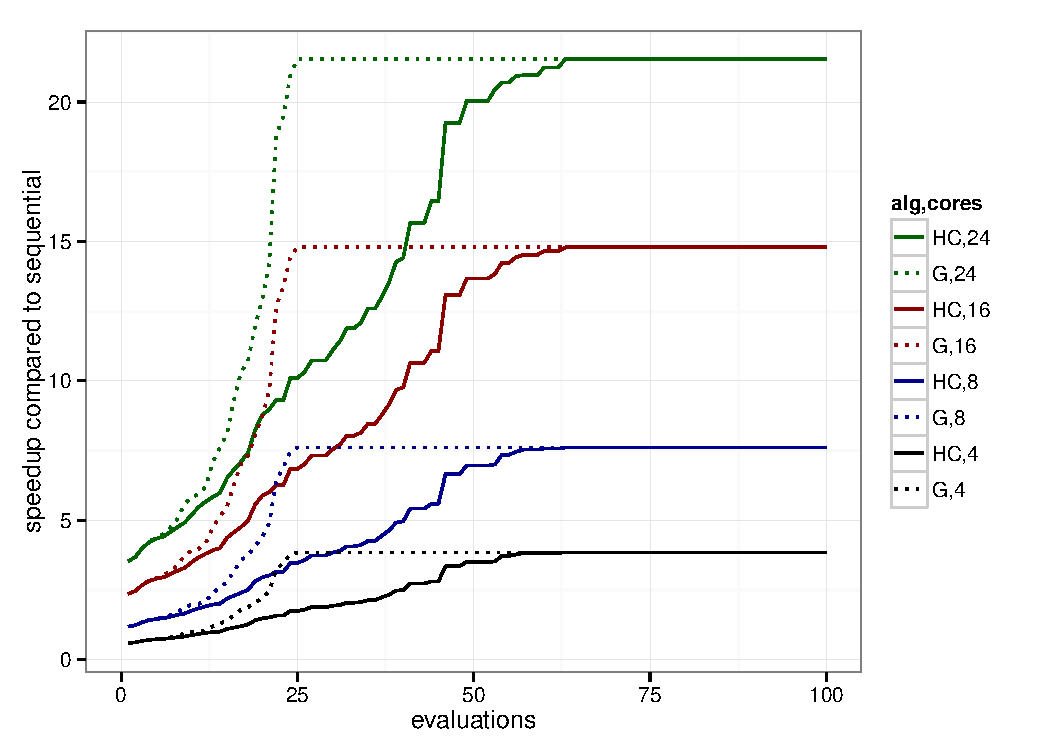
\includegraphics[scale=0.5]{Blind/Figures/speedup_by_evals_Queens2_allon_median.pdf}\\
(a) Queens2\\
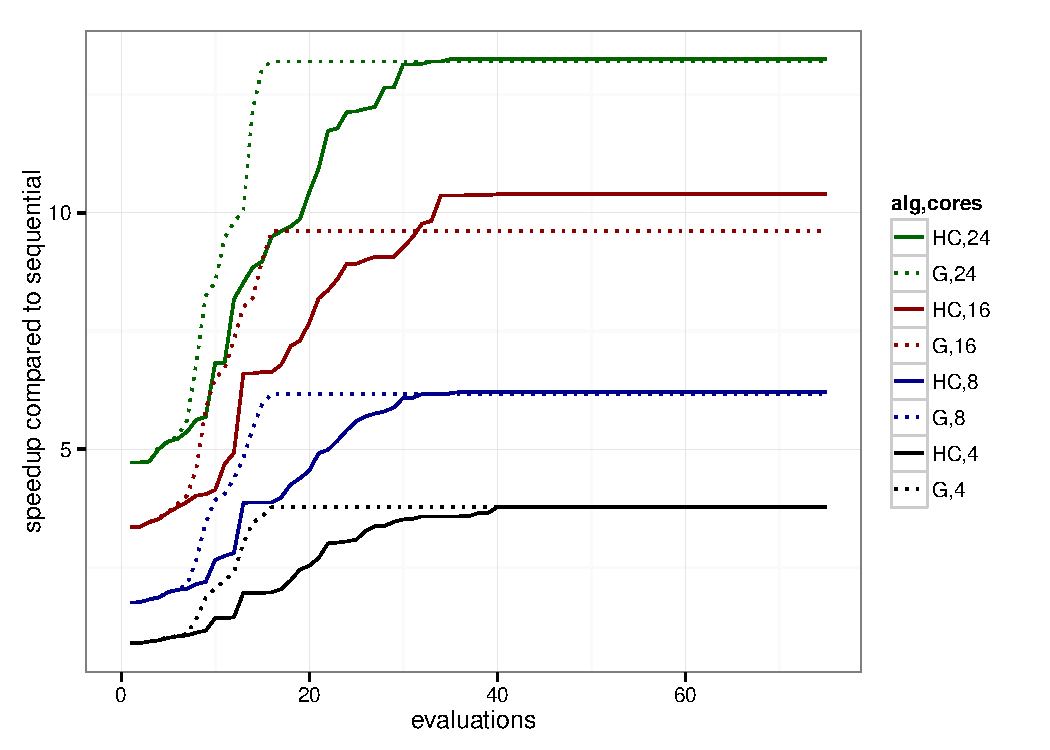
\includegraphics[scale=0.5]{Blind/Figures/speedup_by_evals_SodaCount_allon_median.pdf}\\
(b) SodaCount\\
\caption{The speed-up, calculated as the ratio of the medians of the reduction counts, obtained so far by the algorithm plotted against the number of fitness evaluations. HC and G indicate the hill-climbing and greedy algorithm respectively, both using all-on initialisation. The numbers following the algorithm abbreviation indicate the number of cores.}
\label{fig:evals}
\end{figure}

\paragraph{RQ4} For most SUTs there is no statistically significant difference between all-on and random initialisation.  For SodaCount, the all-on initialisation is slightly better for core counts of 4, 8, and 16.  This result provides evidence that all-on initialisation may be beneficial, but requires further investigation to confirm the generality.

